%mine
\documentclass[12pt,openright,a4paper]{report}
\usepackage{subfigure}
\usepackage{graphicx}
\usepackage{amsmath,amsbsy,amssymb,amsopn}
\usepackage{hyperref}
\usepackage{xcolor}
\usepackage{times}      % times new roman font
\usepackage{fancyhdr}  % Headers and footers
\usepackage[autostyle]{csquotes}% to get double quotes
\usepackage{multirow}


%%%%%%%%%%%%%% To set the page dimension  %%%%%%%%%%%%%%%%%%

\renewcommand{\baselinestretch}{1.2}
\setlength{\textheight}{9.6in} \setlength{\textwidth}{6.4in}
\addtolength{\leftmargin}{-0.3in} \topmargin -.1in
\pagenumbering{}
\addtolength{\topmargin}{-0.5in}
%%%%%%%%%%%%%%%%%%%%%%%%%%%%%%%%%%%%%%%%%%%%
\thispagestyle{empty}

\begin{document}
\begin{center}
{\Large \bf Seminar/ Project Title}

%{\large  S Y N O P S I S}
\vspace{0.55in} {A Seminar/Project Report \\
\emph{Submitted by}\\
{\bf Mr.\; Student Name\\
(13MV010)\\}
 \vspace{0.3in}
To the Savitribai Phule Pune University, Pune\\
 \vspace{0.15in}
\emph{In partial fulfillment for the final examination
of}
}


\vspace{0.3in}

{\bf Bachelor of Engineering}

{\bf In}

{\bf {DEPARTMENT OF COMPUTER ENGINEERING 2021\\

}
 
}


\vspace{0.3in} {\bf{Under the Guidance of}}

{\bf Prof. A.B. CDEF\\} 
\vspace{0.3in}

\begin{figure*}[!h]
\centering
\includegraphics[scale=0.6]{mes.jpg}\\
\end{figure*}
\vspace{0.25cm}
{\bf {DEPARTMENT OF COMPUTER ENGINEERING}}\\
\vspace{0.5cm} {\LARGE{\bf{Modern Education Society's} College of Engineering
\\} }
\vspace{1cm}
{\Large December 2021}
\end{center}
              % input the file my_title.tex           
\newpage
\pagestyle{empty}        %No page number displayed on the pages
\pagestyle{plain}           %To display the page numbers on the pages.
\pagenumbering{roman}
\begin{figure*}[!h]
\centering
\includegraphics[scale=0.4]{mes.jpg}\\
\end{figure*}

\vspace{0.4cm}
\hspace*{-0.5cm}
\begin{center}{\Large \bf {Certificate}}
\end{center}
This is to certify that the thesis entitled:\/  
{\bf{Title of Project}}\/ \/
submitted by \;{\bf{Mr./Ms. Student Name }}
is a bonafide record of the work carried out by him towards the partial fulfillment of
the requirements of Savitribai Pule Pune University, for the final examination of Bachelor of Engineering in Computer Engineering, under my supervision and guidance.\\ \\ 

\vspace*{0.5cm}
\begin{flushright}
Prof. Guide name\\
{\bf{Assistant Professor}}
\end{flushright}

\vspace*{2cm}
\begin{flushright}
Dr. Name of Principal\\
{\bf{Principal}}\\
{\bf{MES COE, Pune-1}}\\
\end{flushright}

\vspace{-2.2cm}
\hspace*{-0.6cm}Dr. Name of HOD\\
{\bf{HOD}}\\
{\bf{Computer Engineering\\}}
Date:\\
Place:\; Pune\\
\hrule
\vspace{0.5cm}
\hspace*{-0.7cm} This report has been examined by us as per the Savitribai Pule Pune University requirements at
{\bf{MES COE, Pune-1 }}on (date):\\

\vspace{0.5cm}
\begin{center}
\hspace*{3.2cm}Signature \\
\hspace*{2.7cm}Name: \\
\hspace*{5cm}{\bf{External Examiner}}\\
\end{center}



\vspace{-2.2cm}
\hspace*{-0.7cm} Signature \\
Name: \\
{\bf{Internal Examiner}} \\


\addcontentsline{toc}{chapter}{Certificate}
\newpage

\begin{center}
{\Large \bf Declaration}
\end{center}
I hereby declare that this submission is my own work and that, to the best of my knowledge and belief, it contains no material previously published or written by another person nor material which has been accepted for the award of any other degree or diploma of the university or other institute of higher learning, except where due acknowledgment has been
made in the text.\\ \\ \\ \\ \\
%\vspace{1cm}
\hspace{-0.1cm}{\bf{Place:\; Pune}}\\ 
{\bf{Date:}}
\vspace{-1.3cm}

\hspace{7.3cm}{\bf{Signature of the Student}}\\
\hspace*{7.8cm} {\bf{Name:}}\\
\hspace*{7.9cm}{\bf{PRN:}}\\




\addcontentsline{toc}{chapter}{Declaration}
\newpage

\begin{center}
{\Large \bf Acknowledgement}
\end{center}


\vspace{5cm}
\begin{flushright}
{\bf{Student name}}
\end{flushright}

\vspace{-1.5cm}
\begin{flushleft}
{\bf{Date:}}
\end{flushleft}
\addcontentsline{toc}{chapter}{Acknowledgement}
\newpage
\begin{center}
{\Large \bf Abstract}\\
\end{center}
The beam steering array antennas,whose radiation pattern can be adjusted in accordance with particular optimum criteria, are called smart antennas. A smart antenna is actually combination of an array of individual antenna elements along with a dedicated signal processing algorithm. The radiation patterns a smart antenna are controlled using algorithms based upon certain criteria. 
\addcontentsline{toc}{chapter}{Abstract}
\newpage

%%%%%%%%%%%%%%%%%%%%%%%%%%%%%%%%%%%%%%%%%%%%%%%
\addcontentsline{toc}{chapter}{Table Of Contents}
\tableofcontents

%%%%%%%%%%%%%%%%
\listoffigures
\addcontentsline{toc}{chapter}{List of Figures}
%%%%%%%%%%%%%%%
\listoftables
\addcontentsline{toc}{chapter}{List of Tables}
%%%%%%%%%%%%%%%%


%Start with the thesis and for this we have to number the page in Arabic numeral, so again need to use pagestyle and pagenumbering.

\newpage
\pagestyle{plain}
\pagenumbering{arabic}
\pagestyle{fancy}
\fancyhf{}
\rhead{Introduction}
\lhead{Chapter 1}
\lfoot{\footnotesize{MES COE, B.E. COMPUTER YEAR 2021-22}}
\rfoot{\thepage}


\chapter{Introduction}


\section{Types}
Following are the different adaptive antenna algorithms \cite{ADR1}:
\begin{enumerate}
\item Least Mean Squares Algorithm. 
\item Sample Matrix Inversion Algorithm.
\item Recursive Least Square Algorithm.
\item Conjugate gradient method.
\item Constant Modulus Algorithm.
\end{enumerate}

\section{Background}

Adaptive Beamforming is a technique in which an array of antennas is exploited to achieve maximum reception in a specified direction by estimating the signal arrival from a desired direction (in the presence of noise) while signals of the same frequency from other directions are rejected.\\
The beamformer array output is given by, 
\begin{equation*}
y(t)= w^{H}\;x(t)
\end{equation*}
the optimum solution for the weight $w_{opt}$ is given by,\\
\begin{equation*}
w_{opt} = R^{-1}\;r
\end{equation*}
where,\; $r = E{[d^*(t)x(t)]}$ is the cross-correlation matrix between the desired signal
and the received signal,\; $R = E[x(t)x^{H}(t)]$ is the auto-correlation matrix of the received signal also known as the covariance matrix.


\section{Objectives}
\begin{itemize}
  \item Formulating the equation of the algorithm.
  \item Algorithm Analysis.
  \item Simulation using MATLAB.
\end{itemize}


\pagestyle{fancy}
\fancyhf{}
\rhead{Fundamentals of Smart Antenna}
\lhead{Chapter 2}
\lfoot{\footnotesize{MES COE, B.E. COMPUTER YEAR 2021-22}}
\rfoot{\thepage}
\chapter{Fundamentals of Smart Antenna}

\section{Introduction}
The term \enquote{smart} refers to the antenna array system that can adapt its radiation pattern according to the need of the user based on a particular criteria. This is done by multiplying each antenna element output by the complex weight that is present in smart antenna system. The complex weight is obtained in many different ways, needs to be adaptive in nature. The adaptation can be achieved when the array is transmitting and receiving \cite{ADR1}.

\section{Smart Antenna}

Smart Antenna systems provide number of significant advantages in wireless communications systems. These include reducing multipath fading, increasing system capacity, increased frequency reuse, sidelobe canceling or null steering, instantaneous tracking of moving sources and the range of a base station. The main functions of smart antennas are: estimation of direction of arrival (DOA) and  beamforming. Algorithms like Capon, MUSIC, ESPRIT, etc. are used for estimating the DOA\cite{ADR1}.


\begin{table}
\begin{center}{\bf \caption{Beamforming Performance Criterion}}
\vspace{1cm}
\begin{tabular}{ |c|c|c| }
\hline
Criterion & No. & Performance \\ \hline 
A & 0 & 55 \\ \hline
B & 1 &  64 \\ \hline
 C& 2 & 47  \\ \hline
 D& 3 & 41 \\
\hline
\end{tabular} 

\end{center}
\end{table}





\section{Beamforming}

The fixed beamforimng algorithm works if the noise and direction of arrival of the desired signals and the interference signals in the environment is not changing. However in practice these may not appear always, so the task of adaptive Beamforming is to estimate the optimal weights for the antenna array system for a rapidly changing environment of channel and DOA. Adaptive Beamforming algorithms have to iteratively estimate the optimum weights to the antenna array system and adapt to the changing signal directions and noise channel states \cite{ADR7}. 

\pagestyle{fancy}
\fancyhf{}
\rhead{Methodology}
\lhead{Chapter 3}
\lfoot{\footnotesize{MES COE, B.E. COMPUTER YEAR 2021-22}}
\rfoot{\thepage}
\chapter{Methodology}

\section{Modelling}

\hspace*{1cm} Here,we have simulated sample-by sample adaptive beam-former using least mean square (LMS) algorithm and constant modulus algorithm (CMA). The weight vector W is calculated using the statistics of signal x(t) arriving from the antenna array.
 An adaptive processor will minimize the error e(t) between a desired signal d(t) and the array output y(t) \cite{ADR3}.



\section{Least Mean Squares}

\hspace*{1cm}
LMS algorithm uses steepest decent method, the output of the steepest decent method is as follows \cite{ADR6} :\\
\vspace*{-1cm}

\begin{equation}
 W(n+1) = W(n)+2\mu E[e(t) x(t)] 
\end{equation}


\noindent
where,  $\mu$ is a gain constant and controls the rate of adaptation. Step size $\mu$  should be chosen in a range in which convergence is ensured  \cite{ADR2}, as,\\
\begin{equation*}
0 < \mu < \frac{2} {\lambda_{max}}
\end{equation*}
where, $\lambda_{max}$ is the largest eigen value of correlation matrix {\emph{R}.\\
Equation (3.1) is the equation of the LMS algorithm \cite{ADR6}.
The weights obtained by the LMS algorithm are only the estimates, but these estimates improve gradually with time as the weights are adjusted for more samples and the filter learns the characteristics of the signals.In practice weight vector 'w' never reaches the theoretical optimum (the Wiener solution i.e. $w_{opt}$), but fluctuates about it.




\pagestyle{fancy}
\fancyhf{}
\rhead{Simulation}
\lhead{Chapter 4}
\lfoot{\footnotesize{MES COE, B.E. COMPUTER YEAR 2021-22}}
\rfoot{\thepage}


\chapter{Simulation}

In the presence of two interfering signals and noise,both amplitude and phase comparison between desired signal and estimated output,beam patterns of the smart antennas and learning characteristics of the above mentioned algorithms are compared and analyzed. In the simulation,the smart antenna of 8 elements has been taken.The smart antenna algorithms compute the antenna weights for all eight antenna elements so that the signal-to-noise-and interference ratio (SINR) becomes optimum\cite{ADR3}.



\section{LMS}
\vspace{-0.5cm}
\begin{figure}[!h]
\hspace{-2.9cm}
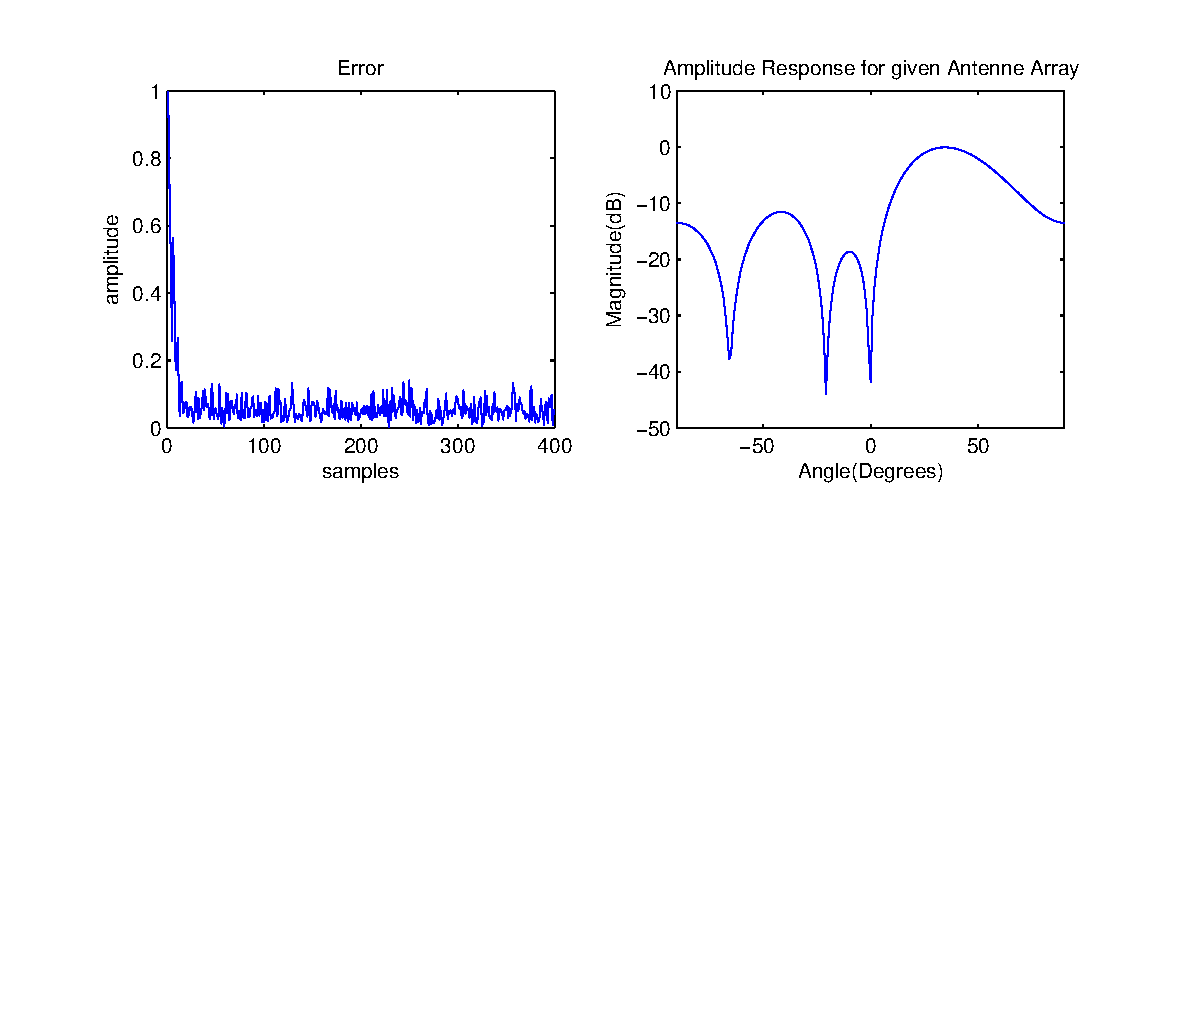
\includegraphics[scale=1.1]{lms1.eps}
\vspace{-10cm}
{\bf{\caption{Error and amplitude response plots for LMS}}}
\end{figure}




\pagestyle{fancy}
\fancyhf{}
\rhead{Conclusion}
\lhead{Chapter 5}
\lfoot{\footnotesize{MES COE, B.E. COMPUTER YEAR 2021-22}}
\rfoot{\thepage}
\chapter{Conclusion}

\begin{itemize}
\item CMA is a blind adaptive beamforming algorithm and LMS is a non-blind adaptive beamforming algorithm. 
\item The advantage of the CMA is the fact that it only needs the instantaneous amplitude of the array output $|y(n)|$ and therefore
no synchronization is required between d and y signals.
\end{itemize}
\addcontentsline{toc}{chapter}{References}

%%%%%%%%%%%%%  Headers and footers %%%%%%%%%%%%%%%%%%%%%%%%
\pagestyle{fancy}
\fancyhf{}
\rhead{References}
\lfoot{\footnotesize{MES COE, B.E. COMPUTER YEAR 2018-19}}
\rfoot{\thepage}
%%%%%%%%%%%%%%%%%%%%%%%%%%%%%%%%%%%%%%%%%%%%%%%

\renewcommand{\bibname}{References} % to write references instead of  bibliography in latex

\begin{thebibliography}{31}
\vspace{-0.6cm}

\bibitem{ADR1}
F. Gross, {\it Smart Antennas For Wireless Communication}, Mcgraw hill,
September 14, 2005.

\bibitem{ADR7}
L.C.Godara, {\it Smart Antennas}, 2004, CRC Press.

\bibitem{ADR8}
H. L. Van Trees, {\it Optimum Array Processing,} Wiley, NY, 2002.

\bibitem{ADR6}
Ifeachor, Emmanuel C., and Barrie W. Jervis. {\it Adaptive Digital Filters. Digital Signal Processing: A Practical Approach.} Second ed. Harlow, England: Prentice Hall, 2002. 650-660. Print.

\bibitem{ADR3}
Das, S., {\enquote{ Smart antenna design for wireless communication using adaptive beam-forming approach,}} {\it TENCON 2008 - 2008 IEEE Region 10 Conference} , vol., no., pp.1,5, 19-21 Nov. 2008.



\end{thebibliography}

\end{document} 